\documentclass[10pt,aspectratio=169, colorlinks=true, linkcolor=circlBlue]{beamer}

% tlp allowed values: clear, green, amber, amber+strict, red
\usetheme[numbering=fraction, progressbar=frametitle]{circl}

% for code highlighting
\usepackage{minted}
% to draw pingus
\usepackage{tikzpingus}
% to draw boxes to catch attention
\usepackage{awesomebox}
% For hyperlinks in the document and PDF metadata
\usepackage{hyperref}
% useful only if we want to customize minted background
\usepackage{tcolorbox}


% set the logo to put in the title page
\titlegraphic{\noindent\hfill
\includegraphics[width=0.3\textwidth]{img/logo-circl.pdf}}
\title{Kunai Introduction}
\subtitle{An Open-Source Threat-Detection Tool for Linux}
\date{2025/07/09}
\author{Quentin JEROME}
\institute{CIRCL Virtual Summer School --- 2025}
\titlelink{\faGithub\space \href{https://github.com/kunai-project}{https://github.com/kunai-project}}

\definecolor{monokaiBackground}{rgb}{0.15, 0.15, 0.15}
% if this is defined globally it will apply to all minted boxes
\tcolorboxenvironment{minted}{
    colback=monokaiBackground, % Use the defined color here
    boxrule=0pt,               % Remove border
    arc=5pt, % Rounded borders
    left=2pt, right=2pt, top=2pt, bottom=2pt % Margins
}


\begin{document}

% Title page
\begin{frame}
	\titlepage%
\end{frame}

\begin{frame}
	\frametitle{Specific Terminology}
	\begin{itemize}
		\item \textbf{Security event}: an event happening on a system which may indicate a potential security incident
		      \begin{itemize}
			      \item[] \textbf{Example}: A log entry that indicates the execution of a given binary
		      \end{itemize}

		\item \textbf{Security monitoring tool}: a tool monitoring a system or an infrastructure and generating security events for analysis.
		      \begin{itemize}
			      \item[] \textbf{Example}: Intrusion Detection Systems (IDS), Endpoint Detection and Response (EDR)
		      \end{itemize}

		\item \textbf{Security visibility}: the ability to monitor,detect and analyze security events
		      \begin{itemize}
			      \item[] \textbf{Example}: A company using a security monitoring software increases its security visibility
		      \end{itemize}

	\end{itemize}
\end{frame}

\begin{frame}
	\frametitle{Different Software for Different Purposes}
	\begin{center}
		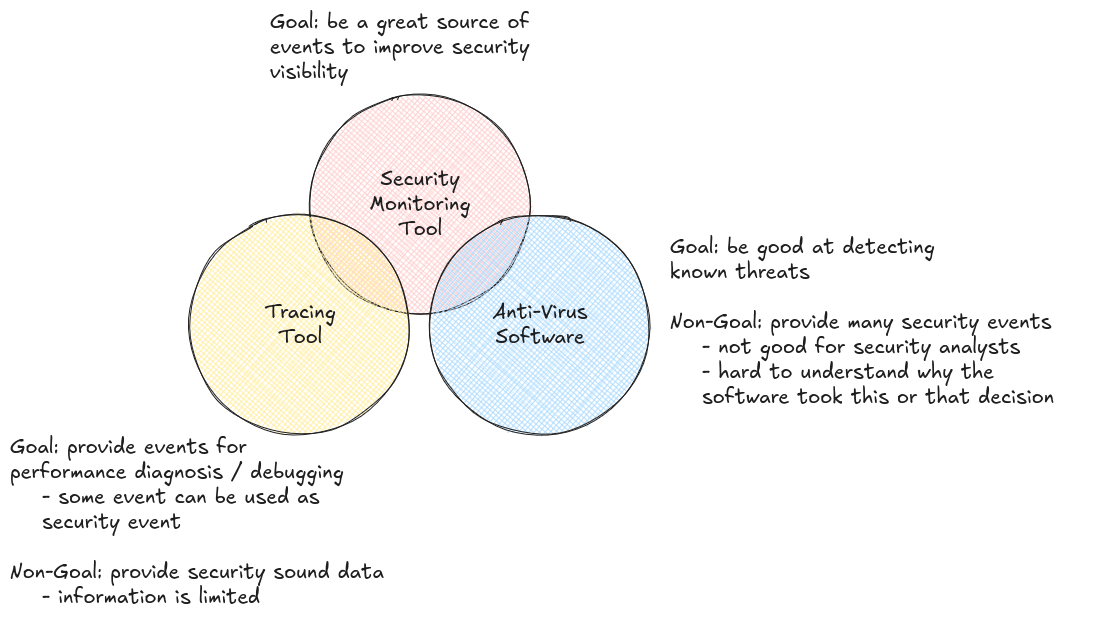
\includegraphics[width=0.9\textwidth]{img/different-tools.png}
	\end{center}
\end{frame}

\begin{frame}
	\frametitle{So What is Kunai?}

	\textbf{Kunai} aims at being a \textbf{Linux} based \textbf{security monitoring} tool helping \textbf{individual/organisations} to increase their \textbf{security visibility} by generating several \textbf{security events}

	\vspace{2em}
	\centering
	A bit more than this actually...%
\end{frame}

\begin{frame}{Brief History}
	\tocinclude

	Project\footnote<.->{\url{https://github.com/kunai-project/kunai}}
	started \textbf{end-2022} as a ``good first Rust project'':

	\textbf{12/2022 - 01/2024}: worked on it under my own company\\
	\textbf{since 01/2024}: joined \textbf{CIRCL} and working on the project
	in the context of an EU co-funded project

	Why starting such a project:

	\begin{itemize}
		\item I was disappointed by \textbf{Sysmon for Linux} for many reasons
		\item Yet there are many good ideas in Sysmon and I think we can do much
		      better by:

		      \begin{itemize}
			      \item
			            getting rid of XML (for configuration and events)
			      \item
			            do not transpose something primarily done for Windows into Linux
		      \end{itemize}
	\end{itemize}
\end{frame}

% What can we do with kunai
\begin{frame}{What can we do with Kunai?}
	\protect\hypertarget{what-can-we-do-with-kunai}{}

	Get high quality \textbf{security events} to perform \textbf{threat detection/hunting}

	\begin{itemize}
		\item
		      Monitor many \textbf{events}\footnote<.->{\href{https://why.kunai.rocks/docs/category/kunai---events}{https://why.kunai.rocks/docs/category/kunai---events}}
		      (execve, shared object loaded, BPF~programs loaded, files
		      read/write/delete \ldots)
		\item
		      Events comes with the following:

		      \begin{itemize}
			      \item
			            Relevant information to build solid \textbf{behavioral detections}
			      \item
			            In chronological order
			      \item
			            Grouping capability through a uuid
			      \item
			            Parent/child tracking
			      \item
			            Enriched with data from previous events (i.e.~network connect/send)
		      \end{itemize}
		\item
		      Accurately track security events generated by \textbf{Linux container} solutions
	\end{itemize}
\end{frame}

% Slide event example
\begin{frame}[fragile]
	\frametitle{Example of execve event}

	\begin{columns}
		\begin{column}{0.5\textwidth}
			\begin{minted}[fontsize=\fontsize{6}{6}\selectfont,style=monokai]{json}
{
  "data": {
    "ancestors": "/usr/lib/systemd/systemd|[...]r/bin/bash",
    "parent_command_line": "bash -ec [...] rm -rf $t; done\"",
    "parent_exe": "/usr/bin/bash",
    "command_line": "mktemp -d -p /tmp/trash",
    "exe": {
      "path": "/usr/bin/mktemp",
      "md5": "0d7660dac3bffd6b76d3054da0fa1216",
      "sha1": "817329148a765bc2dc82baa230638d1987d7a28
4",
      "sha256": "f32938cf25ddd6f6800a8e9b406595534d0eb
27993587bbdeee2e83dd97d8406",
      "sha512": "22d716d4e16492928ec90380d8c6d4749a00
82ffa04630355a1d9a59bd3d196e83169223354a1edd28c5bbec1
37da96ccc6f42558e30cfe2a4d456a0b4c50fba",
      "size": 39144,
      "error": null
    }
  },
  "info": "[...]"
}
			\end{minted}
		\end{column}

		\begin{column}{0.45\textwidth}
			\begin{minted}[fontsize=\fontsize{5}{5}\selectfont,style=monokai]{json}
{
  "data": "...",
  "info": {
    "host": {
      "uuid": "c030b40d-0eab-417b-b33a-22d952357984",
      "name": "hal",
      "container": {
        "name": "ubuntu-kunai-test",
        "type": "docker"
      }
    },
    "event": {
      "source": "kunai",
      "id": 1,
      "name": "execve",
      "uuid": "87f5cb64-11ca-fd34-26af-b47f84132543",
      "batch": 131
    },
    "task": {
      "name": "ls",
      "pid": 1981502,
      "tgid": 1981502,
      "guuid": "cd5415c4-7750-0000-7c85-4ef53e3c1e00",
      "uid": 1000,
      "gid": 1000,
      "namespaces": {
        "mnt": 4026531841
      },
      "flags": "0x400000",
      "zombie": true
    },
    "parent_task": {
      "...": "...",
    },
    "utc_time": "2024-11-19T09:55:53.138247256Z"
  }
}
			\end{minted}
		\end{column}
	\end{columns}
\end{frame}

\begin{frame}[fragile]
	\frametitle{Detection Rules}
	\textbf{Goal}: detect an \textbf{attack/suspicious} pattern

	\centering\begin{minipage}{0.8\textwidth}
		\begin{minted}[fontsize=\fontsize{6}{6}\selectfont,style=monokai]{yaml}
# name of the rule
name: mimic.kthread
# default type is detection so the following line is not mandatory
type: detection
match-on:
    events:
        # we match on kunai execve and execve_script events
        kunai: [execve, execve_script]
matches:
    # 0x200000 is the flag for KTHREAD
    $task_is_kthread: .info.task.flags &= '0x200000'
    # common kthread names 
    $kthread_names: .info.task.name ~= '^(kworker)'
# if task is NOT a KTHREAD but we have a name that 
# looks like one we want the rule to kick-in
condition: not $task_is_kthread and $kthread_names
# severity is bounded to 10 so it is the maximum score
severity: 10
	\end{minted}
	\end{minipage}

	\begin{itemize}
		\item[] Any rule may encode \textbf{actions} to take on a given detection
		      \begin{itemize}
			      \item \textbf{kill}: kill the process triggering the detection
			      \item \textbf{scan-files}: see if file matches malicious \textbf{byte patterns}
		      \end{itemize}
	\end{itemize}

\end{frame}


% Slide event filtering
\begin{frame}[fragile]
	\frametitle{Filtering Rules}

	\begin{columns}
		\begin{column}{0.45\textwidth}
			\textbf{Goals}: save resources \& keep \textbf{context}

			Two ways to filter logs:
			\begin{enumerate}
				\item \textbf{toggle} a \textbf{boolean} switch in configuration
				      \begin{itemize}
					      \item[] Simple and fast, but not granular
				      \end{itemize}
				\item use \textbf{fine grained} filtering
				      \begin{itemize}
					      \item fine granularity
					      \item without context a security alert is \textbf{useless}!
				      \end{itemize}
			\end{enumerate}
		\end{column}

		\begin{column}{0.6\textwidth}
			\begin{minted}[fontsize=\fontsize{6}{6}\selectfont,style=monokai]{yaml}
name: log.mprotect_exec
type: filter
match-on:
    events:
        # applies on kunai mprotect_exec
        kunai: [ mprotect_exec ]
matches:
    # exe matches regex
    $browser: .data.exe.path ~= '/usr/lib/(firefox/firefox|chromium/
chromium)'
# if exe is neither firefox nor chromium
condition: not $browser
	\end{minted}
		\end{column}
	\end{columns}
\end{frame}




\begin{frame}[fragile]
	\frametitle{Raise Alerts on IoCs}

	Indicator of Compromise (\textbf{IoC}): an artifact observed on a network or a system that indicates a computer intrusion

	\begin{itemize}
		\item[] \textbf{Examples}: domain name, IP address, file name, etc.
	\end{itemize}

	Kunai uses a straightforward \textbf{IoC format}

	\centering
	\begin{minipage}{0.6\textwidth}
		\begin{minted}[fontsize=\fontsize{5}{5}\selectfont,style=monokai]{json}
{
  "type": "domain",
  "uuid": "07574cee-4f0e-4fb7-8267-b9dcdbe0c919",
  "source": "CIRCL OSINT Feed",
  "value": "fdh32fsdfhs.shop",
  "severity": 7
}
		\end{minted}
	\end{minipage}

	\begin{enumerate}

		\item
		      kunai perfectly knows which field of its events can be an IoC
		\item
		      so it takes only a few lookups (per events) in a \textbf{hash map}
	\end{enumerate}

	This make \textbf{IoC scanning} very fast and not depending on the
	number of \textbf{IoCs} being loaded
\end{frame}

\section{Integration with other OSS}

\begin{frame}{IoC Provider Integration}
	\protect\hypertarget{ioc-provider-integration}{}
	\begin{itemize}

		\item So far it is integrated with \textbf{MISP}\footnote{\href{https://misp-project.org/}{MISP}} through
		      \textbf{misp-to-kunai.py} \footnote<.->{\href{https://github.com/kunai-project/tools/blob/main/misp/misp-to-kunai.py}{misp-to-kunai.py}}

		      \begin{itemize}
			      \item
			            Can be configured to ingest \textbf{MISP~feeds} (\textbf{no} API key needed)
			      \item
			            Can be configured to export events from a given MISP instance (API
			            key \textbf{required})
			      \item
			            Able to run as a service to regularly pull updates
		      \end{itemize}
	\end{itemize}

	This script lives in a repository\footnote{\href{https://github.com/kunai-project/tools}{kunai tools repository}} where you can find other \textbf{tools} (mainly
	written in Python)
\end{frame}

\begin{frame}{File Scanning Using Yara}

	Recently \textbf{Kunai} has integrated a \textbf{Yara} scanning engine

	What is \textbf{Yara}\footnote{\href{https://virustotal.github.io/yara-x/}{Yara-x project}}:

	\begin{itemize}
		\item a solid project maintained by \textbf{VirusTotal}\footnote{\href{https://virustotal.com}{VirusTotal}}
		\item rule format to \textbf{match patterns} within file
		\item command line tool and a library \textbf{to scan files} with a set of rules
		\item it is a \textbf{well known} format used to share \textbf{malware} detection rules
	\end{itemize}

\end{frame}

\begin{frame}{Integration with Network-Analysis Tools}

	\textbf{Goal}: being able to investigate \textbf{system events} from \textbf{network events} and \textbf{vice versa}

	Corelight designed a \textbf{network flow hashing algorithm} named \textbf{Community ID}\footnote{\href{https://github.com/corelight/community-id-spec}{Community ID specification}}

	Several \textbf{network traffic} analysis tools use it: Corelight / Zeek, Suricata, Wireshark, etc.

	And now \textbf{Kunai} too, in all the network related events it generates

\end{frame}

% Conclusion slide
\section{Conclusions}

\begin{frame}{Takeaways}
	\begin{itemize}
		\item \textbf{Kunai} is an \textbf{open-source} Linux-based security monitoring tool with \textbf{detection capabilities}
		\item Tracks a wide range of \textbf{security events} with detailed context to enable \textbf{behavioral analysis}
		\item Embeds a \textbf{rule engine} to implement \textbf{detection} or \textbf{filtering} rules
		\item Integrates with other \textbf{OSS} projects: \textbf{MISP}, \textbf{Yara}, \textbf{Zeek}, \textbf{Suricata}
		\item \textbf{Kunai} can be used for several purposes:
		      \begin{itemize}
			      \item Enhance \textbf{security visibility}
			      \item Implement \textbf{threat hunting/detection} strategies
			      \item Bring valuable insights for \textbf{incident response}
		      \end{itemize}
	\end{itemize}
\end{frame}

\begin{frame}{Final Words}
	\begin{center}
		\large
		Thank you all for your attention

		It is time to ask questions!
	\end{center}

	\begin{block}{References:}
		\protect\hypertarget{references}{}
		\begin{itemize}

			\item
			      Project: \url{https://github.com/kunai-project/}\\
			\item
			      Documentation: \url{https://why.kunai.rocks/docs/quickstart}
			\item
			      Tools: \url{https://github.com/kunai-project/pykunai}
		\end{itemize}
	\end{block}
\end{frame}

\end{document}% 
